\section{Narzędzia CI/CD}

% W tym rozdziale planuję opisać w jaki sposób tworzone są kompletne pipeline'y, 
% dlaczego są one tak istotne (najlepiej na przykładzie anegdotycznym?).
% Po krótkim wstępie zaprezentuję jak skonfigurowany jest mój pipeline,
% na jakie elementy należy zwrócić uwagę, jaki jest efekt końcowy jego działania.

Zaraz po stworzeniu software'u, najważniejszym etapem jest możliwość szybkiego i bezpiecznego dostarczenia go do odbiorców.
W najmniejszych projektach po skompilowaniu aplikacji zazwyczaj wystarczyło skopiowanie plików
i przeniesienie ich na końcowe urządzenie. O ile jest to najprostsze i najbardziej oczywiste rozwiązanie,
jest ono zdecydowanie najmniej wydajne na dłuższą metę.
\todo[size=\scriptsize]{Czy ten fragment nie jest za mało konkretny? Coś takiego może się znaleźć w pracy dyplomowej?}

\subsection{Wprowadzenie}
Wydanie nowej wersji programu możemy w uproszczony sposób przedstawić jako cykl na poniższym rysunku~\ref{fig:cyklZmian}.
Za każdym razem gdy zostaną wprowadzone jakiekolwiek zmiany, należy przygotować nową wersję (kompilacja),
umieścić ją w odpowiedniej lokalizacji (czy to będzie sklep z aplikacjami, strona internetowa czy nośnik cyfrowy),
a następnie poinformować o tym użytkownika (przykładowo wyświetlić powiadomienie o dostępności aktualizacji).


\begin{figure}[!htp]
    \centering
    \begin{tikzpicture}[
        minimum height=1cm,
        block/.style={rectangle, draw=black!60, fill=green!30, thick, rounded corners=2mm}
        ]
            \node[block] (codeChange) {1. Wprowadzenie zmian w kodzie};
            \node[block] (compilation) [right=of codeChange] {2. Kompilacja rozwiązania};
            \node[block] (publish) [below=of compilation] {3. Publikacja plików};
            \node[block] (newVerInfo) [below=of codeChange] {4. Poinformowanie o nowej wersji};

            \draw[->] (codeChange.east) -- node[anchor=east]{} (compilation.west);
            \draw[->] (compilation.south) -- node[anchor=south]{} (publish.north);
            \draw[->] (publish.west) -- node[anchor=west]{} (newVerInfo.east);
            \draw[dotted] (newVerInfo.north) -- node[anchor=north]{} (codeChange.south);
            
    \end{tikzpicture}
    \caption{Uproszczony proces wydawania nowej wersji oprogramowania}
    \label{fig:cyklZmian}
\end{figure}

Wraz ze wzrostem częstotliwości wprowadzania zmian, ilości urządzeń oraz ograniczeniem dostępu do nich,
potrzeba automatyzacji tego procesu staje się coraz bardziej realna. 
W tym celu wykorzystuje się szeroki wachlarz narzędzi CI/CD. \todo{}

\subsection{Czym jest CI/CD?}
Angielskie \textbf{\textit{Continous Integration / Continous Delivery}} (czyli ciągła integracja i dystrybucja oprogramowania) 
to określenie na zestaw narzędzi automatyzujących dostarczanie programów wraz z ich rozwojem. 
Pełne rozwiązanie, które samodzielnie wypełnia wszystkie nasze kroki wydawcze, nazywamy \textbf{\textit{pipeline}}m (z ang. rurociąg).
Jego istotą jest zapewnienie wydajnego i stabilnego przepływu danych w ramach wypracowanej listy kroków, 
które każdorazowo zostaną wykonane w ten sam sposób~\footnote[1]{
    \label{determinismFootnote}
    Z dokładnością do środowiska, w którym skrypt zostanie uruchomiony, 
    oraz sposobu działania narzędzi (Patrz determinizm kompilatora~\cite{compilerDeterminism})
}, aby otrzymać zamierzony efekt.
Do jego zalet zaliczamy:
\begin{itemize}
    \item Wyeliminowanie błędów i niedopatrzeń człowieka na etapie wydawczym
    \item Przyspieszenie działania procesu
    \item Zwiększenie dostępności 
    \item Determinizm wydania~\footref{determinismFootnote}
    \item Uproszczona analiza szczegółów procesu
\end{itemize}

O ile sam pipeline możemy przedstawić i wykonać jako skrypt terminalowy, 
to jednak dysponujemy już nowoczesnymi narzędziami, które wprowadzają kolejny poziom abstrakcji.
U podstaw są to dokładnie takie same wywołania z linii poleceń, ale opakowanie ich w interfejs graficzny 
upraszcza ich konfigurowanie, obniża trudność uczenia się ich obsługi oraz zazwyczaj pozwala na szybszą analizę 
wyników ich wywołań.

Jako przykład takiego zadania możemy podać skorzystanie .NET Core SDK - o ile musimy poznać możliwości SDK,
to wywołanie ręczne przekazywanie danych wejściowych do terminala zostaje zastąpione modułem, 
dzięki któremu jesteśmy odciążeni z wpisywania słów kluczowych, a jedynie wybieramy je z rozwijanej listy 
lub opisujemy nasze wymagania w skrótach. \todo{To mi brzydko brzmi}

Spotkałem się z opiniami, że przywiązanie do jednego dostawcy narzędzia negatywnie wpływa na elastyczność 
takiego pipeline'a - w przypadku potrzeby zmiany narzędzia CI/CD mogą pojawić się komplikacje, 
przykładowo różnice w składni, limity przechowywania poufnych danych, sposób działania~\footnote[2]{
    Niekompatybilność przekazywania zmiennych, konwencje nazewnicze, dostępność szablonów zadań
} itp.
Aby zabezpieczyć się przed takimi trudnościami, należy przeznaczyć dodatkowe nakłady pracy na stworzenie 
modularnych skryptów, które będą łatwe w użyciu.
Sprawa sekretów jest znacznie bardziej skomplikowana - większość firm stosuje mechanizmy uniemożliwiające pobranie już 
zabezpieczonych danych, więc o ile nie przechowujemy ich kopii samodzielnie, może okazać się to istotnym utrudnieniem w migracji.

Istnieje kilka zagadnień, które należy rozważyć podczas planowania zintegrowania do naszego projektu pipeline'a CI/CD,
czyli podzielonego na kroki procesu, który automatyzuje wspomniane wyżej czynności.
\begin{enumerate}
    \item Ilość czasu potrzebnego do przygotowania konfiguracji

    Chociaż początkowo może wydawać się to zbędnym nakładem pracy, z upływem czasu zwraca się on z nawiązką.
    Jeżeli nasz projekt ma być rozwijany przez więcej osób, w większej perspektywie czasowej, 
    to oprócz jego standardowych zalet, zyskujemy również spokój współautorów, 
    którzy nie muszą znać szczegółów procesu wydawczego i mogą skupić się na tworzeniu jego zawartości.

    Często przygotowanie takiej konfiguracji jest skomplikowane oraz \\ czasochłonne, 
    więc do tego zadania zatrudnia się dobrze zorientowanych specjalistów.

    \item Czy pipeline ma działać w chmurze, czy na własnym urządzeniu

    W zależności od naszych możliwości finansowych oraz zaopatrzeniowych, możemy wynająć maszynę wirtualną
    lub zainstalować odpowiednie oprogramowanie CI/CD na własnej maszynie. 
    Jeżeli wolimy nie martwić się o sprawy sprzętowe, wygodniejszym rozwiązaniem jest chmura,
    ale jeśli dysponujemy sprzętem, to prawdopodobnie skorzystanie z niego będzie tańszą opcją. 
    \todo[size=\scriptsize]{czy ja to muszę jakoś potwierdzać? czy to wystarczy?}
\end{enumerate}


\subsection{Bezpieczeństwo}
Ważnym aspektem jest również bezpieczeństwo - wrażliwe dane, takie jak certyfikaty używane do podpisywania aplikacji czy
hasła dostępowe do serwerów powinny być udostępnione jak najmniejszej ilości osób.

W momencie gdy każdy z deweloperów uaktualnia aplikację ręcznie, musi dysponować tymi informacjami,
zaś korzystając z pipeline'a taki dostęp mają wyłącznie wyselekcjonowane osoby zarządzające procesem.
Zmniejszenie dostępności tych informacji sprawia, że ryzyko wykradnięcia tych danych jest niemal zerowe.

Przykładowo duża firma, która tworzy popularną przeglądarkę internetową, zostaje okradnięta z certyfikatów i haseł - 
będąc w posiadaniu tak istotnych danych, ktoś może stworzyć własną aplikację, która przykładowo wykrada personalia użytkowników, 
a następnie podszyć się pod prawdziwą aplikację. 
Tego rodzaju straty prowadzą do bardzo poważnych konsekwencji, na co nie możemy sobie pozwolić.
\newpage

\subsection{Implementacja}
W mojej pracy zdecydowałem się na skorzystanie z platformy Azure~\ref{MS_AzureSection} - wpłynęły
na nią przyjazny interfejs, łatwość instalacji agenta, jasna struktura tworzenia pipeline'ów 
oraz mnogość instrukcji i poradników dotępnych w Internecie.
\todo[size=\tiny]{Dodać link do rejestracji na Azure (w Dodatkowych linkach)}

Na przykładzie aplikacji Navigator~\ref{NavigatorAppSection} chciałbym przedstawić proces \\
planowania i konfiguracji pipeline'a \todo{}

\subsubsection{Określenie potrzeb i możliwości}
W moim projekcie, oprócz samej kompilacji, postanowiłem zaimplementować etap testowania 
oraz wydania aplikacji na GitHub Releases~\todo{}, czyli publicznej platformie, która 
pozwala na pobranie gotowych programów zgodnych z ich kodem źródłowym. \\
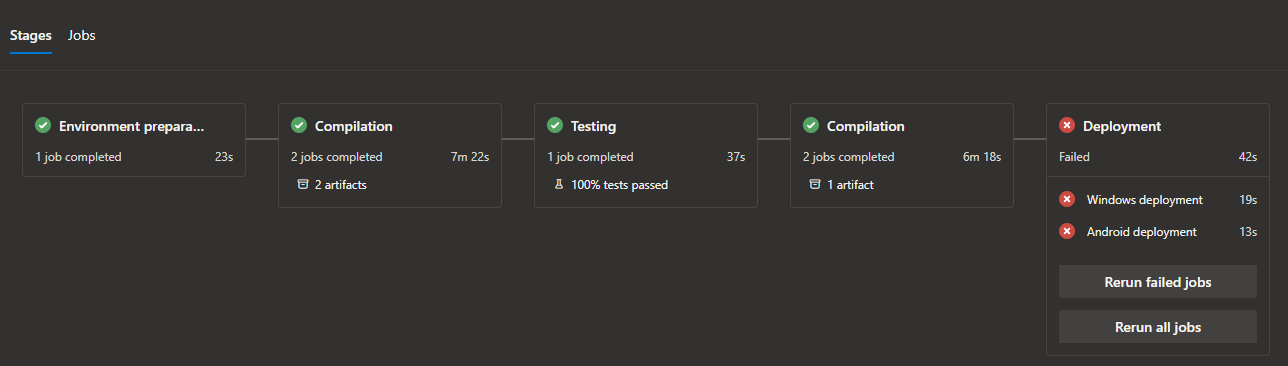
\includegraphics[scale=0.38]{StagesOverview_temp.png}

\subsubsection{Przygotowanie środowiska kompilacyjnego}
Pierwszym krokiem było zainstalowanie specjalnego oprogramowania, 
które wykonuje wszystkie kroki zdefiniowane w pipelinie - Azure Build Agent~\footnote[1]{
    \href{https://learn.microsoft.com/en-us/azure/devops/pipelines/agents/agents}{
        Informacje o Agentach
    }
}.
Ze względu na dysponowanie własną, dostępną maszyną zdecydowałem się na tą opcję,
jednak taki sam efekt można osiągnąć opłacając maszyny wirtualne, udostępniane przez Microsoft.
Po krótkiej konfiguracji\todo{podać tu jakieś szczegóły albo linki?} Agent był gotowy do 
wykonywania zleconego pipeline'owego skryptu, ale należało jeszcze dodać zmienne środowiskowe, 
które pozwalają na skorzystanie z określonych funkcji zadań (przykładem jest użycie Javy~\ref{javaTask}\todo{task java}).

\subsubsection{Zdefiniowanie wymaganych akcji}
Utworzenie pakietu mojej aplikacji napisanej w .NET MAUI przebiega za pomocą wywołania kompilatora 
\verb|dotnet| z opcją \cprotect{\href{https://learn.microsoft.com/en-us/dotnet/core/tools/dotnet-publish}}{\verb|publish|}, 
która uruchamia przywrócenie wszystkich zależności (\verb|restore|), 
kompiluje ją (\verb|build|) oraz pakuje do przewidzianego w konfiguracji projektu (\verb|.csproj|) formatu~\cprotect\footnote{%
    Interesującym może okazać się fakt, że aplikację w .NET MAUI kompilujemy w oparciu o projekt, a nie rozwiązanie (\verb|.sln|).
    Jest to spowodowane mnogością platform, których rozpatrzenie jest 
}.

Zdecydowałem się na podpisywanie aplikacji osobnym zadaniem ze względu na modularność,
jak również ze względu na chęć ominięcia szczegółów tej operacji wewnątrz samego kodu (tj. w pliku projektu).

\subsubsection{Podejście graficzne}
Moja pierwsza próba konfiguracji została podjęta w ramach graficznego konfiguratora, 
który pozwolił mi na wykonanie (jak się później okazało szkicu) 
\label{javaTask}

\subsubsection{Wersja YAML}
Etap kompilacji jest prawie ekwiwalentny do 